\documentclass[12pt]{article}
\usepackage{ctex}
\usepackage{graphicx}  % 用于插入图片
\usepackage{amsmath}  % 数学公式支持
\usepackage{amssymb}  % 额外数学符号支持
\usepackage{listings}  % 用于插入代码
\usepackage{xcolor}  % 代码高亮

\lstset{ 
	language=Matlab,                % 设置代码语言
	basicstyle=\ttfamily\footnotesize, % 设置代码字体
	keywordstyle=\color{blue},    % 设置关键词的颜色
	commentstyle=\color{green},   % 设置注释的颜色
	stringstyle=\color{red},      % 设置字符串的颜色
	breaklines=true,              % 自动换行
	frame=single,                 % 给代码加框
	numbers=left,                 % 显示行号
	numberstyle=\tiny\color{gray}, % 设置行号的样式
	stepnumber=1,                 % 每行代码都显示行号
	xleftmargin=0.3in,            % 设置代码块的左边距
	framexleftmargin=0.3in,       % 设置框的左边距
}

\title{作业一~~拉格朗日插值法实验报告}
\author{姓名: 刘行 \\ 学号: PB22000150}
\date{\today}

\begin{document}
	\maketitle
	\section{实验目的}
		本实验通过拉格朗日插值法对函数 $f(x) = \frac{1}{1+x^2}$ 进行插值逼近, 并比较 \textbf{等距插值点} 与 \textbf{切比雪夫插值点} 的误差情况.

	\section{实验原理}
		拉格朗日插值多项式的数学公式如下:
		\begin{equation}
			p_L(x) = \sum_{i=0}^{N} y_i \ell_i(x),
		\end{equation}
		其中拉格朗日基函数 $\ell_i(x)$ 定义为:
		\begin{equation}
			\ell_i(x) = \prod_{\substack{j=0 \\ j \neq i}}^{N} \frac{x - x_j}{x_i - x_j}.
		\end{equation}

		本实验使用北太天元代码实现该插值过程, 并计算误差:
		\begin{equation}
			\max_{i} |f(y_i) - p_L(y_i)|,
		\end{equation}
		其中插值点选择如下:
		\begin{enumerate}
			\item \textbf{等距节点}: $x_i = 5 - 10i/N$, $i = 0,1,\dots,N$.
			\item \textbf{切比雪夫节点}: $x_i = 5 \cos \left( \frac{(2i+1)\pi}{2N+2} \right)$, $i = 0,1,\dots,N$.
		\end{enumerate}

	\section{代码实现}
		程序主要分为以下几个部分:
		\begin{enumerate}
			\item 定义目标函数 $f(x)$;
			\item 计算拉格朗日插值多项式;
			\item 选择不同的插值节点;
			\item 计算插值误差并输出.
		\end{enumerate}

		其中拉格朗日插值多项式由函数 \texttt{lagrange\_interpolation} 给出, 具体实现如下:
		\begin{lstlisting}[language=Matlab]
lagrange_interpolation = @(x, y, xi) ...
	sum(arrayfun(@(i) y(i+1) * ...
	prod((xi - x([1:i, i+2:end])) ./ ...
	(x(i+1) - x([1:i, i+2:end]))), 0:length(x)-1));
		\end{lstlisting}

		在计算 $N = 10$ 的插值多项式之后将图像输出.

	\section{程序使用说明及实验结果}
		本程序在北太天元软件中编写, 在北太天元界面中直接执行:
		\begin{verbatim}
			>> lagrange
		\end{verbatim}
		输出结果:
		\begin{verbatim}
N=5
Max Error of grid (1) : 0.4326923077
Max Error of grid (2) : 0.5559113388
N=10
Max Error of grid (1) : 1.9156430502
Max Error of grid (2) : 0.1089290399
N=20
Max Error of grid (1) : 58.2781251077
Max Error of grid (2) : 0.0153250885
N=40
Max Error of grid (1) : 78689.0374853696
Max Error of grid (2) : 0.0002738598
		\end{verbatim}

		对应 $N = 10$ 的函数与插值多项式图像如下:
		\begin{figure}[htbp]
			\centering
			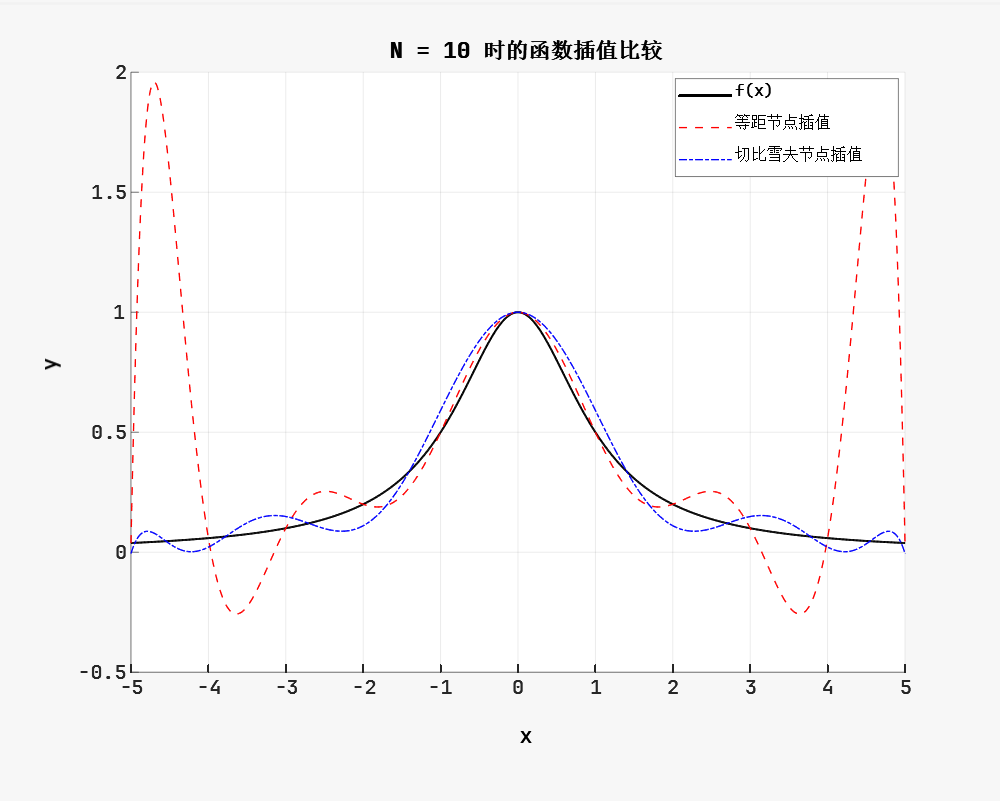
\includegraphics[width=0.5\textwidth]{interpolation.png}
			\caption{N=10 时的拉格朗日插值比较}
			\label{fig:interpolation}
		\end{figure}

	\section{实验分析}
	从实验结果可以观察到:
	\begin{enumerate}
		\item \textbf{插值误差随 $N$ 增大而减小}, 但等距节点仍存在较大误差, 甚至随着 $N$ 的增大有所增加.
		\item 当 $N = 40$ 时, 切比雪夫插值误差已经非常小, 而等距插值仍然存在较大偏差.
		\item \textbf{切比雪夫节点具有更好的数值稳定性}.
	\end{enumerate}

	\section{结论}
	本实验验证了拉格朗日插值法在不同插值节点下的误差变化情况。结果表明, \textbf{切比雪夫节点优于等距节点}, 能有效减少误差, 提高插值精度.
\end{document}
